The last two sections introduced the selection to suppress photons originating in non-\mbox{\BtoXsgamma} decays, particularly from \piz and \eta decays (\Cref{sec:photon_selection}),
and the strategy suppress \mbox{\epem\ra\qqbar} events which were the dominant component in the selected data set (\Cref{sec:continuum_suppression}).
Although a preselection was already developped to prepare an adequate training sample for the \BDT, a more optimal (`tighter') selection is desired to ensure the optimal efficiency and purity of the selected sample.
This section will describe the approach taken to find this optimal selection, and calculate the efficiency loss for all applied selections.

\subsection{Simultaneous selection optimisation}\label{sec:simultaneous_optimisation}

After the pre-selection that prepared the data for training a \BDT in \Cref{tab:preselections}, a more robust strategy for tighter selections is developed.
In particular, \BDT output, \piVeto, \etaVeto and \ZMVA may be interconnected, in the sense that applying the selection on one of them, may influence a selection on the others. 
To find an optimal selection point, each selection is optimised in an iteration-based approach, 
where each requirement is optimised to a value that gives best figure-of-merit score individually,
while keeping the other requirements unvaried.
The individual optimisation are equivalent to that shown in \Cref{fig:selection_optimisations} and use figure-of-merit $\mathtt{FOM}_2$ defined in \Cref{eq:punzi_fom}.


In order to maximise the efficiency of events on kinematically well-reconstructed events, without adhering to a more strict definition at this stage, 
this procedure is performed on peaking events ($\Mbc >5.27~\gevcc$) and a single combination of the highest energy photon with a randomly selected tag-candidate per event.
The starting point for each selection correspond to values in \Cref{tab:preselections}.
The starting $\mathtt{BDT~output}$ selection is chosen at 0.5. 
The \BtoXsgamma admixture of charged and neutral modes is used.
The \epem\ra\qqbar and generic \BB background events from \feiBp and \feiBz modes are merged.
This aims to reproduce `realistic' data conditions, where different efficiencies may be related due to different \FEI and selection behaviour on charged and neutral modes.

After performing the optimisation for each selection, the optimisation round is repeated 9 more times.
The selections converge and do not vary after round 3 optimisation.
The converged value that is found is shown in \Cref{tab:interative_optimisation}.

\begin{table}[htbp!]
    \centering
    \caption{\label{tab:interative_optimisation} Optimal selections chosen for this analysis, based on the iterative approach described in \Cref{sec:simultaneous_optimisation}.
    The values for $\mathtt{BDT~output}$ and \ZMVA are chosen near those that are found optimal.
    For \piVeto and \etaVeto the choice is made based on the availability of data-simulation agreement studies performed at Belle II.
    At the time of preparing the analysis, 
    only studies with \piVeto and \etaVeto thresholds 
    up to 0.4 were analyses and appropriate correction factors supplied (see \Cref{sec:piz_eta_calibration}).
    }
    \begin{tabular}{|l|c|c|}
        \hline
        Variable &    Figure-of-merit maximised at & Final chosen \\
        \hline
        \ZMVA                      & $>0.629$ & 0.6\\
        \piVeto                    & $<0.258$ & 0.4\\
        \etaVeto                   & $<0.036$ & 0.4\\
        $\mathtt{BDT~output}$      & $>0.798$ & 0.8\\
        \hline
\end{tabular}
\end{table}

For \piVeto and \etaVeto, the found selection is relatively tight, if inspecting \Cref{fig:bp_piveto,fig:bz_piveto,fig:bp_etaveto,fig:bz_etaveto}.
Furthermore, at the time of preparation of the analysis desribed, studies regarding the \piVeto and \etaVeto applicability to such tight selections were not done.
Therefore, it was decided to not tighten this selection further than the pre-selection value obtained in \Cref{tab:preselections}.
Repeating the study while keeping \piVeto and \etaVeto selection at 0.4 yields compatible results to those shown in \Cref{tab:interative_optimisation}.
Therefore, other selections are chosen based on the optimal value from the initial 10 iterations.

\subsection{Summary and efficiency of all analysis selections}\label{sec:selection_summary}

A table, summarising all the selections and \BDT training results from \Cref{sec:photon_selection,sec:continuum_suppression,sec:final_optimisation},
and listing the final \BtoXsgamma candidate retention, is shown in \Cref{tab:cutflow}.
The retention, in this case, is defined as:
\begin{equation}\label{eq:loose_efficiency}
    r_{\mathrm{cand}} = \frac{N_{\BtoXsgamma}~\mathrm{candidates~after~cut}}{N_{\BtoXsgamma}~\mathrm{no~cut}},
\end{equation}
which is an estimate, as it may include multiple tag-side $B$ candidates.
For the calculation of this table, the $\Mbc>5.27~\gevcc$ requirement is no longer applied and all tag-$B$ meson candidates are maintained (i.e. high-energy photon candidates may contribute more than once per event).

\begin{table}[htbp!]
    \centering
    \caption{\label{tab:cutflow} The summary table of all selections and their retentions, based on \Cref{eq:loose_efficiency}.
    The selections listed here are applied on official Belle II \feiBp and \feiBz samples, described in \Cref{sec:reconstruction_overview}.
    The columns show efficiency costs for \BtoXsgamma events, calculated on signal \MC, continuum and \BB events, both of which are calculated on generic \MC.
    It can be seen that continuum events are suppressed by roughly two orders of magnitude, whereas generic-\BB decays -- by more than an order of magnitude.
    }
    \centering
\begin{minipage}[c]{0.49\textwidth}
    \centering
    \feiBp mode reconstruction
    \resizebox{1\textwidth}{!}{
        \begin{tabular}{lrrr}
            \multirow{2}{*}{Selection}   & \BtoXsgamma & Continuum &    \BB events \\
                                         & \multicolumn{3}{c}{Retention}     \\       
            \hline                                        
            none                  & 1.0000 & 1.0000    & 1.0000 \\
            $E_{\gamma}$ rank $= 1$     & 0.9979 & 0.9660    & 0.9762 \\
            $\ZMVA>0.6$        & 0.9435 & 0.6543    & 0.6957 \\
            $\piVeto<0.4$ & 0.8309 & 0.2145    & 0.3140 \\
            $\etaVeto<0.4$  & 0.9212 & 0.7637    & 0.7676 \\
            $\mathtt{BDT~output}>0.8$   & 0.5615 & 0.0253    & 0.4854 \\
            tag-$\Mbc>5.245~\gevcc$         & 0.9485 & 0.8863    & 0.9287 \\
            \hline
            all                   & 0.4211 & 0.0045    & 0.0731 \\
            \end{tabular}
            
    }
\end{minipage}
\begin{minipage}[c]{0.49\textwidth}
    \centering
    \feiBz mode reconstruction
    \resizebox{1\textwidth}{!}{
        \begin{tabular}{lrrr}
            \multirow{2}{*}{Selection}   & \BtoXsgamma & Continuum &    \BB events \\
                                         & \multicolumn{3}{c}{Retention} \\
            \hline 
            none                  &1.0000 & 1.0000 & 1.0000 \\
            $E_{\gamma}$ rank $= 1$     &0.9982 & 0.9680 & 0.9791 \\
            $\ZMVA>0.6$        &0.9449 & 0.6570 & 0.6899 \\
            $\piVeto<0.4$ &0.8411 & 0.2221 & 0.3235 \\
            $\etaVeto<0.4$  &0.9272 & 0.7824 & 0.7739 \\
            $\mathtt{BDT~output}>0.8$  &0.5538 & 0.0251 & 0.4791 \\
            tag-$\Mbc>5.245~\gevcc$          &0.9461 & 0.8837 & 0.9230 \\
            \hline
            all                   &0.4206 & 0.0047 & 0.0735 \\
            \end{tabular}
    }
\end{minipage}
\end{table}

\Cref{tab:cutflow} shows that the background suppression procedure roughly halves the number of available \BtoXsgamma events in the sample.
However, the background candidates from \epem\ra\qqbar processes are reduced 200 times, to less than 0.5\% of the original value.
Furthermore, generic-\BB event contribution is estimated at about 7\% of the original, which means more than an order of magnitude suppression is achieved.
The photon energy spectrum, after these selections have been applied is shown in \Cref{fig:spectrum_after_optimisation}.
Compared with previous iterations of this figure, e.g.\Cref{fig:spectrum_after_reco}, a much better signal-to-background ratio is clearly visible.

\begin{figure}[htbp!]
    \centering
    \subcaptionbox{\label{fig:spectrum_after_optimisation_bp}}{
        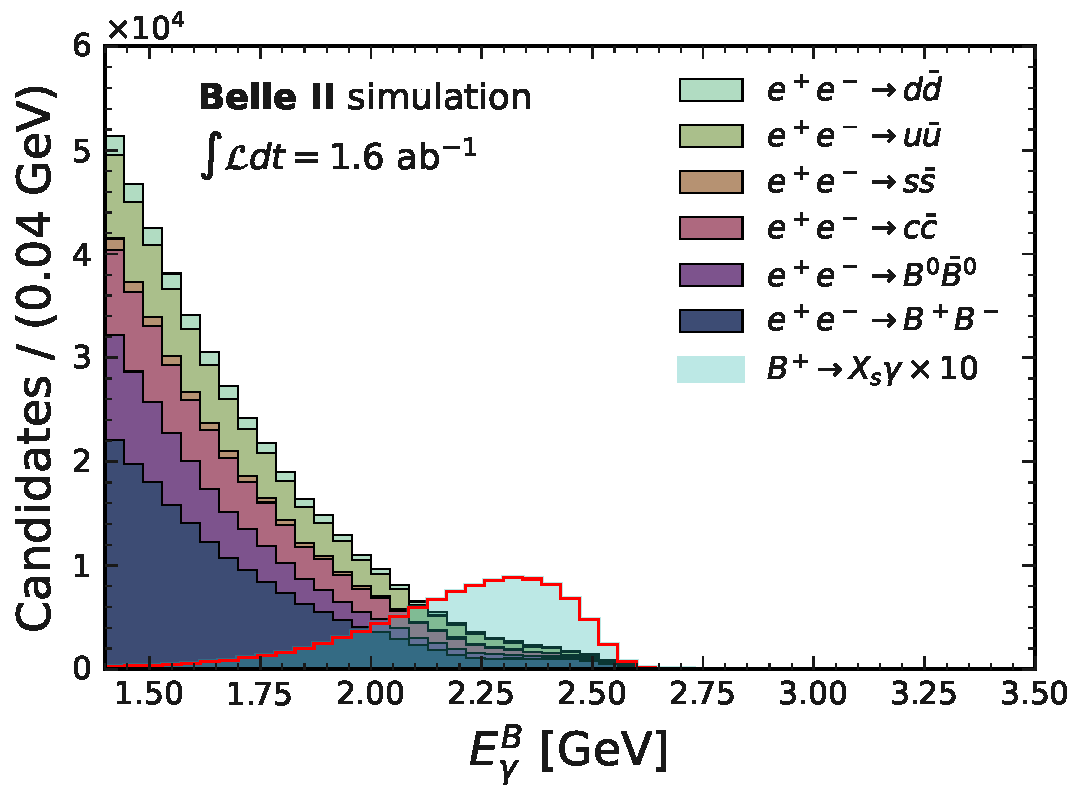
\includegraphics[width=0.4\textwidth]{figures/final_optimisation/Bp_tagged_background_optimal.pdf}
    }    
    \subcaptionbox{\label{fig:spectrum_after_optimisation_bz}}{
        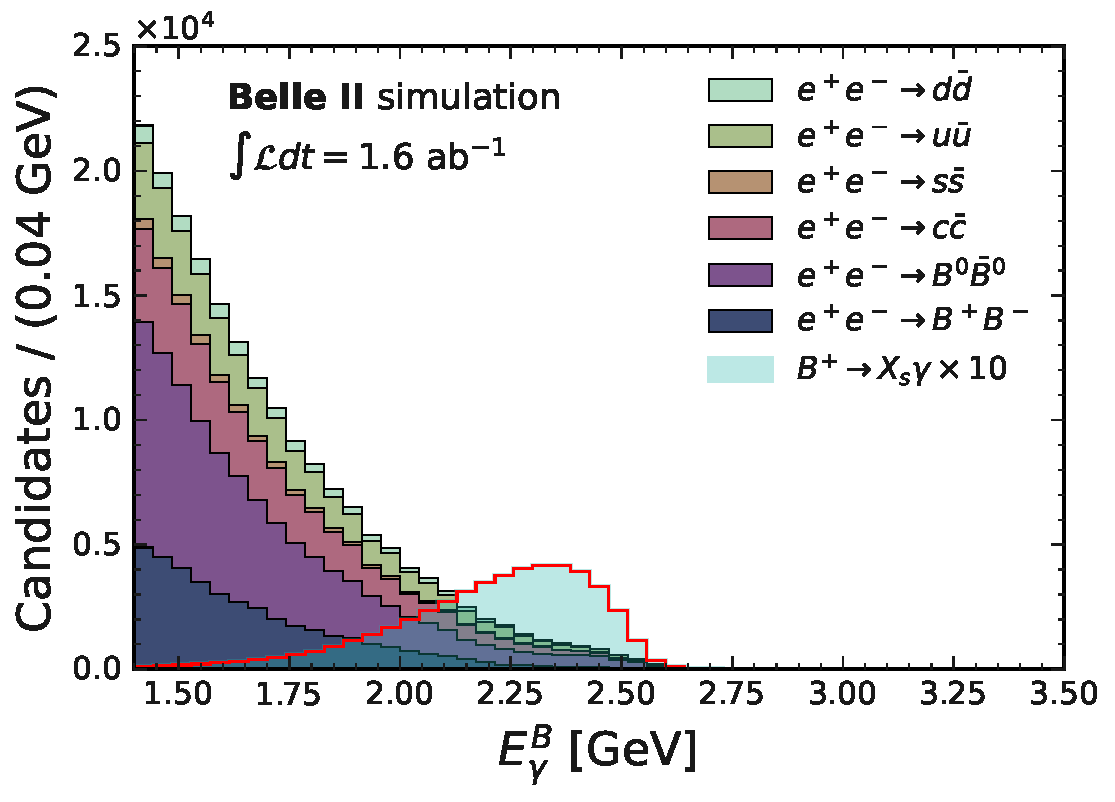
\includegraphics[width=0.4\textwidth]{figures/final_optimisation/Bz_tagged_background_optimal.pdf}
    }    
    \caption{\label{fig:spectrum_after_optimisation}\BtoXsgamma spectrum in generic \MC after event reconstruction and optimised selections applied, lised in \Cref{tab:cutflow}.
    Overlaid are events from signal \MC where the photon comes from \BtoXsgamma, multiplied by a scaling factor, with the same selections applied.
    These figures may include a high-energy photon combined with multiple tag entries per event and can be compared directly with \Cref{fig:spectrum_after_reco}.
    Compared to the post-reconstruction figure, the scaling factor for \BtoXsgamma is 100 times lower.}
\end{figure}
